% This file was created with tikzplotlib v0.10.1.
\begin{tikzpicture}

\definecolor{darkorange25512714}{RGB}{255,127,14}
\definecolor{darkslategray38}{RGB}{38,38,38}
\definecolor{lightgray204}{RGB}{204,204,204}
\definecolor{steelblue31119180}{RGB}{31,119,180}

\begin{axis}[
axis line style={lightgray204},
height=0.45\textheight,
legend cell align={left},
legend style={fill opacity=0.8, draw opacity=1, text opacity=1, draw=none},
tick align=outside,
tick pos=left,
title={Performance vs. Productivity in C++ and Rust for HPC},
width=\textwidth,
x grid style={lightgray204},
xlabel=\textcolor{darkslategray38}{Estimated cost of development [\$]},
xmajorgrids,
xmin=10161.2, xmax=47182.8,
xtick style={color=darkslategray38},
y grid style={lightgray204},
ylabel=\textcolor{darkslategray38}{Total runtime for 200x200x200 mesh [s]},
ymajorgrids,
ymin=6.4475, ymax=71.4025,
ytick style={color=darkslategray38}
]
\path [draw=black, semithick]
(axis cs:11844,57.5)
--(axis cs:11844,58.7);

\path [draw=black, semithick]
(axis cs:11980,11.73)
--(axis cs:11980,11.81);

\path [draw=black, semithick]
(axis cs:27553,58.23)
--(axis cs:27553,58.33);

\path [draw=black, semithick]
(axis cs:27723,68.07)
--(axis cs:27723,68.45);

\path [draw=black, semithick]
(axis cs:31665,43)
--(axis cs:31665,44.2);

\path [draw=black, semithick]
(axis cs:31970,9.4)
--(axis cs:31970,10.2);

\path [draw=black, semithick]
(axis cs:45180,48.63)
--(axis cs:45180,48.73);

\path [draw=black, semithick]
(axis cs:45500,35.7)
--(axis cs:45500,36.04);

\addplot [semithick, black, mark=x, mark size=3, mark options={solid,draw=steelblue31119180}, only marks]
table {%
11844 58.0999984741211
11980 11.7700004577637
27553 58.2799987792969
27723 68.2600021362305
};
\addlegendentry{C++}
\addplot [semithick, black, mark=x, mark size=3, mark options={solid,draw=darkorange25512714}, only marks]
table {%
31665 43.5999984741211
31970 9.80000019073486
45180 48.6800003051758
45500 35.8699989318848
};
\addlegendentry{Rust}

\draw (axis cs:11944,58.1) node[
  scale=0.4165,
  anchor=base west,
  text=black,
  rotate=0.0
]{serial};
\draw (axis cs:12080,11.77) node[
  scale=0.4165,
  anchor=base west,
  text=black,
  rotate=0.0
]{rayon};
\draw (axis cs:27653,58.28) node[
  scale=0.4165,
  anchor=base west,
  text=black,
  rotate=0.0
]{mpi};
\draw (axis cs:27823,68.26) node[
  scale=0.4165,
  anchor=base west,
  text=black,
  rotate=0.0
]{hybrid};
\draw (axis cs:31765,43.6) node[
  scale=0.4165,
  anchor=base west,
  text=black,
  rotate=0.0
]{serial};
\draw (axis cs:32070,9.8) node[
  scale=0.4165,
  anchor=base west,
  text=black,
  rotate=0.0
]{openmp};
\draw (axis cs:45280,48.68) node[
  scale=0.4165,
  anchor=base west,
  text=black,
  rotate=0.0
]{mpi};
\draw (axis cs:45600,35.87) node[
  scale=0.4165,
  anchor=base west,
  text=black,
  rotate=0.0
]{hybrid};

\end{axis}
\end{tikzpicture}
